\documentclass[12pt,letterpaper]{article}
\usepackage[utf8]{inputenc}
\usepackage{tikz}
\usetikzlibrary{trees}
\usepackage[spanish, es-nodecimaldot]{babel}
\usepackage{amsmath}
\usepackage{color}
\usepackage{algorithm}
\usepackage[noend]{algpseudocode}
\renewcommand{\algorithmicrequire}{\textbf{Entrada:}}
\renewcommand{\algorithmicensure}{\textbf{Salida:}}
\usepackage{subcaption}
\usepackage{amsfonts}
\usepackage{hyperref}
 \hypersetup{
     colorlinks=true,
     linkcolor=blue,
     filecolor=blue,
     citecolor = blue,      
     urlcolor=cyan,
     }
\usepackage{amssymb}
\usepackage{listings}
\usepackage{color}

\newcommand\var[1]{\, \mathrm{Var}\left\lbrack #1 \right\rbrack}

\newcommand\cov[1]{\, \mathrm{Cov} \left\lbrack #1 \right\rbrack}
\newcommand\pr[1]{\, P \left( #1 \right)}

\newcommand\esp[1]{\, \mathbb{E} \left\lbrack #1 \right\rbrack}
\newcommand\integral[4]{\ensuremath{\int_{#1}^{#2} #3 \, d#4}}

\definecolor{mygreen}{rgb}{0,0.6,0}
\definecolor{mygray}{rgb}{0.5,0.5,0.5}
\definecolor{mymauve}{rgb}{0.58,0,0.82}

\lstset{ 
  backgroundcolor=\color{white},   % choose the background color; you must add \usepackage{color} or \usepackage{xcolor}; should come as last argument
  basicstyle=\footnotesize,        % the size of the fonts that are used for the code
  breakatwhitespace=false,         % sets if automatic breaks should only happen at whitespace
  breaklines=true,                 % sets automatic line breaking
  captionpos=b,                    % sets the caption-position to bottom
  commentstyle=\color{mygreen},    % comment style
  deletekeywords={...},            % if you want to delete keywords from the given language
  escapeinside={\%*}{*)},          % if you want to add LaTeX within your code
  extendedchars=true,              % lets you use non-ASCII characters; for 8-bits encodings only, does not work with UTF-8
  firstnumber=1,                % start line enumeration with line 1000
  frame=single,	                   % adds a frame around the code
  keepspaces=true,                 % keeps spaces in text, useful for keeping indentation of code (possibly needs columns=flexible)
  keywordstyle=\color{blue},       % keyword style
  language=R,                 % the language of the code
  morekeywords={*,...},            % if you want to add more keywords to the set
  numbers=none,                    % where to put the line-numbers; possible values are (none, left, right)
  numbersep=5pt,                   % how far the line-numbers are from the code
  numberstyle=\tiny\color{mygray}, % the style that is used for the line-numbers
  rulecolor=\color{black},         % if not set, the frame-color may be changed on line-breaks within not-black text (e.g. comments (green here))
  showspaces=false,                % show spaces everywhere adding particular underscores; it overrides 'showstringspaces'
  showstringspaces=false,          % underline spaces within strings only
  showtabs=false,                  % show tabs within strings adding particular underscores
  stepnumber=2,                    % the step between two line-numbers. If it's 1, each line will be numbered
  stringstyle=\color{mymauve},     % string literal style
  tabsize=2,	                   % sets default tabsize to 2 spaces
  title=\lstname                   % show the filename of files included with \lstinputlisting; also try caption instead of title
}

\usepackage{amsthm}
\newtheorem{theorem}{Teorema}

\usepackage{graphicx}
\usepackage[inner=1.5 cm, outer = 1.5 cm, top=1 cm, bottom = 1.5 cm]{geometry}
\setlength{\parskip}{3mm}
\title{\textsc{Ley de los grandes números}}
\author{\textsc{Fabiola Vázquez}}

\setlength{\parindent}{0cm}
\renewcommand{\lstlistingname}{Código}
\floatname{algorithm}{Algoritmo}
\newtheorem{ej}{Ejercicio}
\newtheorem{defi}{Definición}
\newtheorem{teo}{Teorema}



\begin{document}
\maketitle
\hrule 
\section{Introducción}
 En el presente trabajo se aborda la ley de los grandes números. Primero, se presentan algunos resultados teóricos preliminares, seguido de la demostración \cite{snell} de la ley de los grandes números. Así mismo, se enuncia la ley fuerte de los grandes números. Finalmente, se habla del método de Monte-Carlo como una aplicación de los resultados teóricos previos.
\section{Ley de los grandes números}
\begin{teo}
Si $X$ es una variable aleatoria no negativa, entonces para $\varepsilon > 0$ se tiene que
\begin{equation}
P(X\geqslant \varepsilon) \leqslant \frac{\esp{X}}{\varepsilon}.
\end{equation}
\end{teo}

\begin{teo}
Si $X$ es una variable aleatoria no negativa, entonces, para todo $\varepsilon > 0$ y para todo entero positivo $n$, se tiene 
\begin{equation}
P(X \geqslant \varepsilon) \leqslant \frac{\esp{X^n}}{\varepsilon^n}.
\end{equation}
\end{teo}
\begin{proof}[Demostración]
Se considera la desigualdad 
\begin{equation}
X \geqslant \varepsilon.
\end{equation}
Elevando ambos lados de la desigualdad a la potencia $n$, se tiene que
\begin{equation}
X^n \geqslant \varepsilon^n.
\end{equation}
Entonces, es claro que
\begin{equation}
P(X \geqslant \varepsilon) = P(X^n \geqslant \varepsilon^n),
\end{equation}
donde $X^n$ es una variable aleatoria no negativa, ya que $X$ es no negativa. Por el teorema anterior, se tiene que
\begin{equation}
P(X^n \geqslant \varepsilon^n) \leqslant \frac{\esp{X^n}}{\varepsilon^n}.
\end{equation}
Por lo tanto,
\begin{equation}
\label{basica}
P(X \geqslant \varepsilon) \leqslant \frac{\esp{X^n}}{\varepsilon^n}.
\end{equation}
\end{proof}
\begin{teo}[Desigualdad de Chebyshev]
Sea $X$ una variable aleatoria discreta con valor esperado $\esp{X}=\mu$, y sea $\varepsilon > 0$ cualquier número real positivo. Entonces,
\begin{equation}
P\left(|X-\mu| \leqslant \varepsilon \right) \leqslant \frac{\var{X}}{\varepsilon^2}
\end{equation}
\end{teo}
\begin{proof}[Demostración]
Se considera la variable aleatoria $|X-\esp{X}|$ y la ecuación \ref{basica} con $n=2$, se tiene
\begin{equation}
P(|X-\esp{X}|\geqslant \varepsilon) \leqslant \frac{\mathbb{E}\left[\mid X - \esp{X}\mid ^2 \right]}{\varepsilon^2}.
\end{equation}
Como $\var{X} = (X - \esp{X})^2$, se tiene que
\begin{equation}
P(|X-	\esp{X}|\geqslant \varepsilon) \leqslant \frac{\var{X}}{\varepsilon^2}.
\end{equation}
\end{proof}

\begin{teo}[Ley de los grandes números \cite{snell}]
Sea $X_1, X_2, \ldots $ un proceso independiente de ensayos con valor esperado finito $\mu = \esp{X_{i}}$ y varianza finita $\sigma^2 = \var{X_{j}}$. Sea $S_{n} = X_1 + X_2 + \ldots + X_n$. Entonces para cualquier $\varepsilon >0$,
\begin{equation}
P\left(\frac{S_n}{n} - \mu \geqslant \varepsilon \right) \longrightarrow 0
\end{equation}
cuando $n\longrightarrow \infty$. Equivalentemente,
\begin{equation}
P \left( \frac{S_n}{n} - \mu < \varepsilon \right) \longrightarrow 1
\end{equation}
cuando $n \longrightarrow \infty.$
\end{teo}
\begin{proof}[Demostración]
Dado que $X_1, X_2, \ldots, X_n$ son variables aleatorias independientes con las mismas distribuciones, se tiene que 
\begin{equation}
\var{S_n} = n \sigma^2,
\end{equation}
y
\begin{equation}
\var{\frac{S_n}{n}} = \frac{\sigma^2}{n}. 
\end{equation}
Como $\esp{\frac{S_n}{n}}=\mu$ y por la desigualdad de Chebyshev, se tiene que par cualquier $\varepsilon > 0$
\begin{equation}
\pr{\left\vert \frac{S_n}{n} - \mu \right\vert \geqslant \varepsilon} \leqslant \frac{\sigma^2}{n\varepsilon^2}.
\end{equation}
Como 
\begin{equation}
\lim\limits_{n \rightarrow \infty} \frac{\sigma^2}{n\varepsilon^2} = 0
\end{equation}
y $\pr{\left\vert \frac{S_n}{n} - \mu \right\vert \geqslant \varepsilon} \geqslant 0$, por lo tanto
\begin{equation}
\lim\limits_{n\rightarrow \infty} \pr{\left\vert \frac{S_n}{n} - \mu \right\vert \geqslant \varepsilon} = 0.
\end{equation} 
Equivalentemente, 
\begin{equation}
\lim\limits_{n \rightarrow \infty} \pr{\left\vert \frac{S_n}{n} - \mu \right\vert \geqslant \varepsilon} = 1.
\end{equation}
\end{proof}

\begin{teo}[Ley fuerte de los grandes números \cite{stochastic_simulation}]
Sea $X_1, X_2, \ldots, X_n$ una secuencia de variables aleatorias independientes e idénticamente distribuidas, tales que $\esp{X_i} < \infty$. Para $N \geqslant 1$, se denota la media empírica de $X_1, X_2, \ldots, X_n$ por
\begin{equation}
\hat{S}_N := \frac{1}{N} \sum^{N}_{i = 1} X_i.
\end{equation}
Entonces,
\begin{equation}
\lim\limits_{N \longrightarrow \infty} \hat{S}_N = \esp{X_i}.
\end{equation}
\end{teo}

\section{Método de Monte-Carlo}
Una de las aplicaciones de la ley de los grandes números es la aproximación de integrales definidas \cite{stochastic_simulation}. Suponga que se tiene una función $f(x)$ y se busca el valor $\varphi$ donde 
\begin{equation}
\varphi = \int_{0}^{1} f(x) dx.
\end{equation}
Por la definición de valor esperado se sabe que 
\begin{equation}
\varphi = \esp{f(U)}
\end{equation}
si $U \sim \mathrm{Unif}(0,1)$. Si $U_1, \ldots, U_k$ son variables aleatorias independientes distribuidas uniformemente en $(0,1)$, se sigue que $f(U_1), \ldots, f(U_k)$ son variables aleatorias independientes idénticamente distribuidas con media $\varphi$. Entonces, por la ley fuerte de los grandes números, se sigue que, con probabilidad 1, 
\begin{equation}
\sum^{n}_{i=1} \frac{f(U_{i})}{n} \longrightarrow \esp{f(U)} = \varphi
\end{equation}
cuando $n \longrightarrow \infty$. Por lo tanto, se puede aproximar $\varphi$ generando una cantidad grande de números pseudo aleatorios $u_i$ y tomando como aproximación la media de los valores de $f(u_i)$. Este método para aproximar integrales es llamado el método de Monte-Carlo.

Para aproximar cualquier integral sobre el intervalo $[a,b]$ se puede modificar la integral que se tenía en el intervalo $[0,1]$ con el cambio de variable $x=a+(b-a)u$, es decir
\begin{equation}
\int_a^b f(x) dx = (b-a)\int^1_0 f(a+(b-a)u)du \approx \frac{b-a}{N}\sum^N_{i=1}f(a+(b-a)u_i), 
\end{equation}
donde $u_i$ son variables aleatorias uniformemente distribuidas en $[0,1]$.

Como ejemplo, se quiere estimar el valor de la integral,
\begin{equation}
\label{integral}
\int^1_0 \frac{x}{e^x + e^{-x}} \, dx.
\end{equation}
Para ello se genera una cantidad de números pseudo aleatorios, cada uno se evalúa en la función $f(x)=\frac{x}{e^x+e^{-x}}$, se suman los resultados y se divide entre la cantidad de números. Esto se realiza con el código \ref{lst:function} en el software R \cite{R}. 

La figura \ref{im} muestra como el valor obtenido con el método de Monte-Carlo se aproxima al valor real (línea roja) cuando la cantidad de números pseudo aleatorios aumenta.
\begin{lstlisting}[caption = Función para aproximar una integral con el método de Monte-Carlo., label={lst:function}]
f <- function(x) { return(x/(exp(x)+exp(-x)) }

mc.integral <- function(f, cuantos){
    A <- runif(cuantos)
    return(sum(f(A))/cuantos)
}
\end{lstlisting}

\begin{figure}
\centering
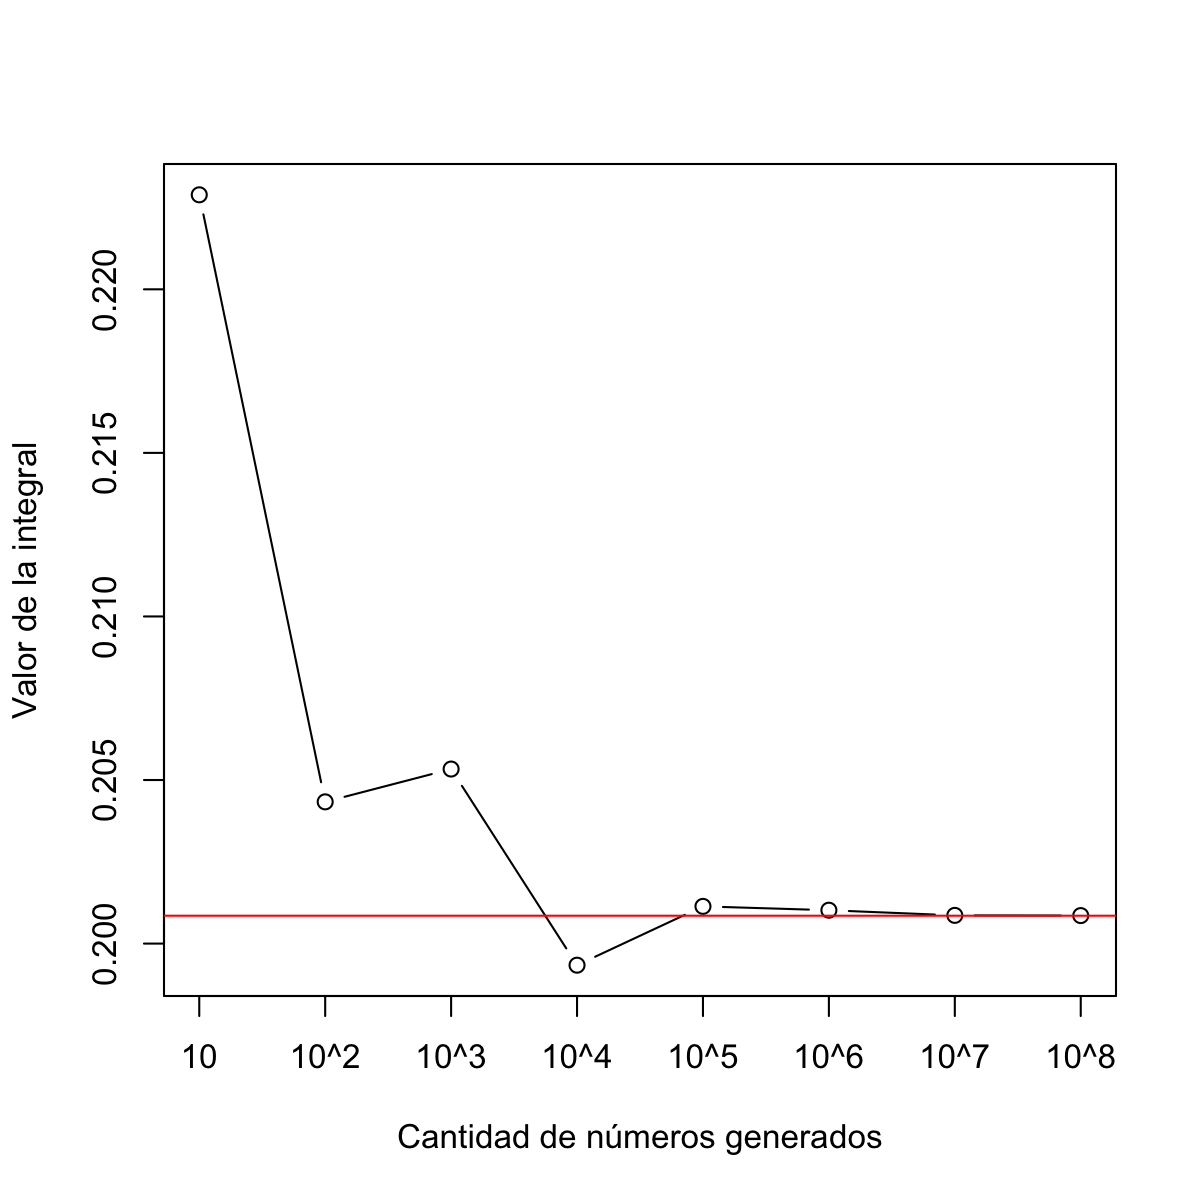
\includegraphics[scale=0.3]{int1.png}
\caption{Aproximación de la integral \ref{integral} mediante el método de Monte-Carlo. }
\label{im}
\end{figure}

\bibliographystyle{plain} 
\bibliography{ref}
\end{document} 